%
%===============>>  ГРУППА 6-2 МОДУЛЬ 6  <<=============
%
\setmodule{6}

%BEGIN_FOLD % ====>>_____ Занятие 1 _____<<====
\begin{class}[number=1-2]
	\title{Занятие 1}
	\begin{listofex}
		\item Вычислить:
		\begin{tasks}(2)
			\task \( 3,12+\dfrac{1}{4} \)
			\task \( 5,404+\dfrac{13}{25} \)
			\task \( \mfrac{3}{4}{50}-1,57\)
			\task \( \mfrac{2}{1}{10}+2,2 \)
			\task \( \mfrac{4}{1}{7}+1,66 \)
			\task \( \mfrac{12}{13}{15}-10,6 \)
			\task \( \mfrac{2}{5}{18}-1,1\)
			\task \( \mfrac{1}{1}{3}+35,7 \)
		\end{tasks}
		\item Вычислить:
		\begin{tasks}(4)
			\task \( 1,5 : \dfrac{1}{3} \)
			\task \( \dfrac{3}{8} : 0,25 \)
			\task \( 3,2 \cdot \dfrac{5}{8} \)
			\task \( 3,6 \cdot \mfrac{2}{7}{9} \)
			\task \( \mfrac{5}{2}{5} \cdot  \mfrac{2}{7}{9} \)
			\task \( \mfrac{2}{11}{12} \cdot 0,1 \)
			\task \( 1,45 : \mfrac{2}{1}{3} \)
			\task \( 20 : \mfrac{33}{1}{3} \)
		\end{tasks}
		\item Вычислить:
		\begin{tasks}(1)
			%\task \( \left(  \mfrac{2}{3}{4} + \mfrac{4}{1}{8} \right) \cdot \mfrac{1}{5}{11} \)
			\task \( 16 \cdot \left( \mfrac{5}{8}{21} - \mfrac{3}{79}{84} \right) + 15 \cdot \left( \dfrac{1}{2} + \mfrac{2}{1}{3} \cdot \mfrac{1}{4}{5} \right) \)
			\task \( \left( \mfrac{1}{2}{13} \cdot 0,42 + 0,78 \cdot \mfrac{1}{2}{13} \right) \cdot \mfrac{1}{4}{9} : 0,6 - 0,5 \cdot \mfrac{5}{2}{3} \)
		\end{tasks}
		\item В четырех домах \(567\) жителя. В одном доме \(\dfrac{1}{3}\) всех жителей, во втором --- в \(1,5\) раза меньше, чем в первом, а остальные живут поровну в третьем и четвёртом домах. По скольку жителей живёт в третьем и четвёртом домах?
	\newpage
	\title{Занятие 2}
	\end{listofex}
	\begin{definit}
		Сумма внутренних углов в треугольнике равна \( 180\degree \).
	\end{definit}
	\begin{definit}
		\textbf{Внешний угол} --- угол между стороной треугольника и продолжением другой стороны. Внешний угол является смежным с одним из внутренних.
	\end{definit}
	\begin{listofex}
		\item В треугольнике \( ABC \) два угла равны \( 50\) и \( 70 \) градусов. Найдите третий угол.
		\item Один угол треугольника равен \( 26\degree \), а второй в три раза больше. Найдите третий угол.
		\item Один внутренний угол треугольника в два, а второй в три раза больше третьего, найдите все углы треугольника.
		\item Один внешний угол равен \( 40\degree \), а второй --- \( 100\degree \). Чему равны внутренние углы треугольника?
		\item Угол треугольника равен \( 30\degree \), второй угол в \( 3 \) раза больше первого. Чему равны внешние углы при каждой вершине? Чему равна сумма внешних углов?
		\item В прямоугольном треугольнике один угол равен \( 40 \) градусов. Найдите сумму наибольшего и наименьшего угла.
		\item В прямоугольном треугольнике один острый угол на \( 17 \) градусов больше другого. Найдите углы треугольника.
		\item В прямоугольном треугольнике два острых угла равны. Какая у них градусная мера?
	\end{listofex}
\end{class}
%END_FOLD

%%BEGIN_FOLD % ====>>_____ Занятие 2 _____<<====
%\begin{class}[number=2]
%	\begin{listofex}
%		\item Занятие 2
%	\end{listofex}
%\end{class}
%%END_FOLD

%BEGIN_FOLD % ====>>_ Домашняя работа 1 _<<====
\begin{homework}[number=1]
	\begin{listofex}
		\item В треугольнике \( ABC \) два угла равны \( 130\) и \( 15 \) градусов. Найдите третий угол.
		\item Один угол треугольника равен \( 31\degree \), а второй в четыре раза больше. Найдите третий угол треугольника.
		\item Один внешний угол равен \( 15\degree \), а второй --- \( 120\degree \). Чему равны внутренние углы треугольника?
		\item В прямоугольном треугольнике один острый угол равен \( 32 \) градуса. Найдите сумму наибольшего и наименьшего угла.
		\item Вычислить:
		\begin{tasks}(2)
			\task \( 3,12+\dfrac{1}{4} \)
			\task \( 5,404-\mfrac{4}{21}{25} \)
			\task \( \mfrac{1}{5}{12}-1,3\)
			\task \( 4 : \dfrac{10}{4} \)
			\task \( \dfrac{1}{8} \cdot 4,25 \)
			\task \( 1,5 \cdot \dfrac{2}{3} \)
			\task \( \left(  \mfrac{1}{5}{6} + \mfrac{2}{11}{12} \right) \cdot 12 \)
		\end{tasks}
		\item \( (*) \) \(4\) кузнеца должны подковать \(5\) лошадей. Каждый кузнец тратит на одну подкову \(5\) минут. Какое наименьшее время они должны потратить на работу? Учтите, что лошадь не может стоять на двух ногах.
	\end{listofex}
\end{homework}
%END_FOLD

%BEGIN_FOLD % ====>>_____ Занятие 3 _____<<====
\begin{class}[number=3-4]
	\title{Занятие 3}
	\begin{listofex}
		\item
		\begin{minipage}[t]{\bodywidth}
			Определите координаты точек:
		\end{minipage}
		%\hspace{0.02\linewidth}
		\begin{minipage}[c]{0.45\textwidth}
			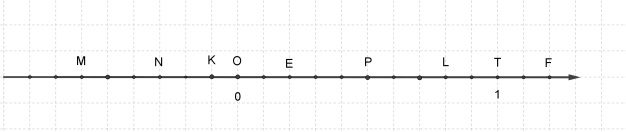
\includegraphics[align=t, width=\linewidth]{\picpath/G61M6L1-1}
		\end{minipage}
	\end{listofex}
	\begin{definit}
	Чтобы вычесть из отрицательного числа отрицательное число, нужно сложить их так, будто они положительные, а перед суммой поставить минус.
	\end{definit}
	\begin{listofex}[resume]
		\item Вычислите:
		\begin{tasks}(4)
			\task \( -28-14 \)
			\task \( -144-56 \)
			\task \( -9-17 \)
			\task \( -3-18 \)
			\task \( -12-7 \)
			\task \( -15-8 \)
			\task \( -24-19 \)
			\task \( -8-3 \)
		\end{tasks}
	\end{listofex}
	\begin{definit}
		Для удобства, при сложении отрицательного числа с положительным, сумму можно записать как разность, поставив положительное число перед отрицательным. \\ Например, \(-12+25=25-12=13\).
	\end{definit}
	\begin{listofex}[resume]
		\item Вычислите:
		\begin{tasks}(4)
			\task \( -35 + 92 \)
			\task \( -7+14 \)
			\task \( -17+21 \)
			\task \( -5+65 \)
			\task \( -26+27 \)
			\task \( -8+12 \)
			\task \( -32+32 \)
			\task \( -80+124 \)
		\end{tasks}
	\end{listofex}
	\begin{definit}
		Если перед скобками стоит знак минус, то при их раскрытии знак внутри скобок меняется на противоположный. \\ Например: \(-(-a) = a \) или \( -(b) = -b \)
	\end{definit}
	\begin{listofex}[resume]
		\item Вычислите:
		\begin{tasks}(3)
			\task \( -35 - (-42) \)
			\task \( 8-(6) \)
			\task \( -(19)-(-21) \)
			\task \( -5-(-27) \)
			\task \( -(-42)+18 \)
			\task \( -(-17)-26 \)
			\task \( -(-29)+(-13) \)
			\task \( -(18)+(-12) \)
		\end{tasks}
	\end{listofex}
	\begin{definit}
		Чтобы из меньшего числа вычесть большее, необходимо из большего вычесть меньшее и перед результатом поставить знак минус. \\ Например: \( 17-82 = -(82-17)=-65 \)
	\end{definit}
	\begin{listofex}[resume]
		\item Вычислите:
		\begin{tasks}(4)
			\task \( 15-21 \)
			\task \( 17-66 \)
			\task \( 100-143 \)
			\task \( 42-69 \)
			\task \( 85-98 \)
			\task \( 117-162 \)
			\task \( 31-67 \)
			\task \( 71-143 \)
		\end{tasks}
		\item Вычислите:
		\begin{tasks}(2)
			\task \( -\mfrac{2}{3}{7}-\mfrac{3}{5}{14} \)
			\task \( -\mfrac{4}{8}{9}+\mfrac{6}{7}{15} \)
			\task \( -3,3+\mfrac{4}{8}{7} \)
			\task \( -5,6+\mfrac{5}{3}{5} \)
			\task \( 9,9-\mfrac{11}{4}{15} \)
			\task \( -\mfrac{8}{4}{23}+\mfrac{9}{5}{46}+\left(-\mfrac{18}{13}{69}\right) \)
			\task \( -2,3 + \left(-\mfrac{1}{3}{5}\right) + 9,09 \)
			\task \( -\mfrac{6}{8}{12} + \left(-\dfrac{13}{24}\right) - (-7,11) \)
		\end{tasks}
		\item В прямоугольном треугольнике один угол в два раза меньше другого. Какими могут быть эти углы?
	\end{listofex}
	\title{Занятие 4}
	\begin{listofex}
		\item
		\begin{minipage}[t]{\bodywidth}
			Определите координаты всех точек:
		\end{minipage}
		%\hspace{0.02\linewidth}
		\begin{minipage}[c]{0.7\linewidth}
			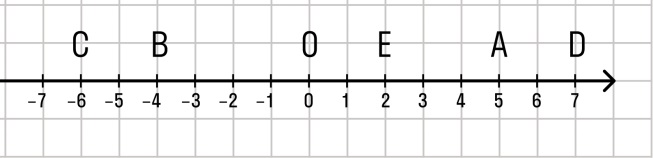
\includegraphics[align=t, width=\linewidth]{\picpath/G61M6L2-1}
		\end{minipage}
	\end{listofex}
	\begin{definit}
		Рациональные числа, как и целые, можно сравнивать с помощью числовой оси --- \textbf{чем правее расположено число, тем оно больше.}
	\end{definit}
	\begin{listofex}[resume]
		\item С помощью этого же рисунка сравните координаты точек:
		\begin{tasks}(3)
			\task \( A \) и \( D \)
			\task \( B \) и \( C \)
			\task \( B \) и \( E \)
			\task \( O \) и \( B \)
			\task \( E \) и \( C \)
			\task \( O \) и \( C \)
		\end{tasks}
		\newpage
		\item Сравните рациональные числа:
		\begin{tasks}(3)
			\task \( -5 \) и \( -3 \)
			\task \( -7 \) и \( -25 \)
			\task \( 4 \) и \( -1 \)
			\task \( -99 \) и \( -101 \)
			\task \( -10,5 \) и \( -1,5 \)
			\task \( -8,9 \) и \( -9,2 \)
			\task \( -55,3 \) и \( -55,4 \)
			\task \( -0,2 \) и \( 0 \)
			\task \( \dfrac{1}{3} \) и \( -\dfrac{1}{4} \)
			\task \(- \dfrac{4}{7} \) и \( \dfrac{3}{4} \)
			\task \(- \mfrac{1}{3}{15} \) и \( -\dfrac{3}{15} \)
			\task \( -\mfrac{2}{3}{4} \) и \( -\dfrac{2}{5} \)
		\end{tasks}
		\item Вычислите:
		\begin{tasks}(3)
			\task \( -\dfrac{5}{9}-\dfrac{5}{9} \)
			\task \( -\dfrac{14}{15}+\dfrac{5}{6} \)
			\task \( -\dfrac{1}{2}-\dfrac{1}{3} \)
			\task \( \mfrac{3}{5}{6}-4 \)
			\task \( -1,18+\dfrac{33}{50} \)
			\task \( -0,8+4 \)
			\task \( 1,7-7,3 \)
			\task \( -2,4+3,6 \)
			\task \( -5,7-2,15 \)
		\end{tasks}
	\end{listofex}
	\begin{definit}
	Модулем положительного числа называется само число. \\
	Модулем отрицательного числа называется противоположное ему число. \\
	Модуль нуля равен нулю.
	\end{definit}
	\begin{listofex}[resume]
		\item Найдите модуль:
		\begin{tasks}(3)
			\task \(  |3| \)
			\task \(  |-15| \)
			\task \( |-14|  \)
			\task \( |-1,5|  \)
			\task \(  \left|-\mfrac{4}{5}{6}\right| \)
			\task \(  \left|\dfrac{-1}{4}\right| \)
			\task \(  \left|-\dfrac{-8}{15}\right| \)
			\task \(  \left|-\mfrac{7}{8}{9}\right| \)
			\task \(  \left|-\dfrac{28}{-9}\right| \)
		\end{tasks}
		%\item У нас было  \(115\)  рублей, в первом магазине потратили \(\dfrac{2}{5}\) этой суммы, а потом еще \(\dfrac{8}{10}\) от остатка. Сколько денег мы потратили и сколько денег у нас осталось?
		%\item В четырех домах \(567\) жителя. В одном доме \(\dfrac{1}{3}\) всех жителей, во втором --- в \(1,5\) раза меньше, чем в первом, а остальные живут поровну в третьем и четвёртом домах. По скольку жителей живёт в третьем и четвёртом домах?
		%\item Из одного центра управления запущены три беспилотника для видеосъемки акватории Азовского моря. Время съемки первого --- \(8\) мин, второго --- \(12\) мин, а третьего --- \(18\) мин. Через какое время беспилотники одновременно вернуться в центр управления, если их запускают вновь после очередной перезарядки?
		\item Решите пропорции:
		\begin{tasks}(2)
			\task \( \dfrac{x}{24}=\dfrac{15}{6} \)
			\task \( 14:x=5:8\)
		\end{tasks}
	\end{listofex}
\end{class}
%END_FOLD

%%BEGIN_FOLD % ====>>_____ Занятие 4 _____<<====
%\begin{class}[number=4]
%	\begin{listofex}
%		\item Занятие 4
%	\end{listofex}
%\end{class}
%%END_FOLD

%BEGIN_FOLD % ====>>_ Домашняя работа 2 _<<====
\begin{homework}[number=2]
	\begin{listofex}
		\item Вычислите:
		\begin{tasks}(2)
			\task \( -11 + 21 \)
			\task \( -17+25 \)
			\task \( -37+65 \)
			%\task \( -51-14 \)
			\task \( -26-37 \)
			\task \( -83-22 \)
			\task \( -\dfrac{1}{3}+\dfrac{1}{2} \)
			\task \( -\mfrac{2}{1}{6}+11 \)
			\task \( -1,5-\dfrac{3}{7} \)
			%\task \( -\mfrac{3}{5}{21}+\mfrac{3}{17}{42}+\left(-\mfrac{18}{45}{66}\right) \)
			\task \( -15,2 + \left(-\mfrac{2}{17}{25}\right) + 12 \)
			\task \( -\mfrac{4}{2}{3} + \left(-\dfrac{22}{24}\right) - (-6) \)
			\task \(  |-15,2|-\left|-\mfrac{5}{13}{25}\right| \)
			%\task \(  -|\dfrac{-5}{8}|-|\dfrac{-3}{4}| \)
			\task \(  -\left|\dfrac{-18}{9}\right| + |-7,5-|-1,2|| \)
		\end{tasks}
		\item Сравните рациональные числа:
		\begin{tasks}(3)
			\task \( -\dfrac{1}{2} \) и \( -\dfrac{3}{4} \)
			%\task \( -\dfrac{5}{11} \) и \( -\dfrac{6}{33} \)
			\task \( -\mfrac{1}{5}{7} \) и \( -\dfrac{13}{8} \)
			%\task \( -11,5 \) и \( -17,22 \)
			\task \( -8,85 \) и \( -8,02 \)
			%\task \( -14,4 \) и \( -14,02 \)
		\end{tasks}
		\item Найдите модуль:
		\begin{tasks}(3)
			\task \(  |18| \)
			\task \(  |-22| \)
			\task \( |-1,5|  \)
			\task \(  \left|-\mfrac{2}{1}{3}\right| \)
			\task \(  \left|\dfrac{-1}{-5}\right| \)
			\task \(  \left|-\dfrac{-3}{25}\right| \)
		\end{tasks}
	\end{listofex}
\end{homework}
%END_FOLD

%BEGIN_FOLD % ====>>_____ Занятие 5-6 _____<<====
\begin{class}[number=5-6]
	\begin{definit}
		Модулем положительного числа называется само число. \\
		Модулем отрицательного числа называется противоположное ему число. \\
		Модуль нуля равен нулю.
	\end{definit}
	\begin{listofex}
		\item Найдите модуль:
		\begin{tasks}(3)
			\task \(  |3| \)
			\task \(  |-15| \)
			\task \( |-76,5|  \)
			\task \( |-14+5,2|  \)
			\task \( |-22,1-5,7|  \)
			\task \(  \left|2-\mfrac{4}{5}{6}\right| \)
			\task \(  \left|\dfrac{-1}{4}\right| \)
			\task \(  \left|\dfrac{-8}{15}\right| \)
			\task \(  \left|\mfrac{1}{5}{26}\right| \)
			\task \(  \left|-\dfrac{11}{-3}\right| \)
			\task \(  \left|-\dfrac{-15}{2}\right| \)
			\task \(  \left|-\dfrac{14}{-|-55|}\right| \)
		\end{tasks}
		\item Вычислите:
		\begin{tasks}(2)
			\task \(  |-5|+|-11| \)
			\task \(  -|-15|-|11,5| \)
			\task \( |-8,3|-|-5| \)
			\task \( |-2,3|+|3,7|  \)
			\task \(  |-10|\cdot|-15| \)
			\task \(  -|-9,6|\cdot|-17| \)
			\task \( |-4,7|:|-1,9| \)
			\task \( |-21+32,5| - \left|\dfrac{-3}{5}\right|  \)
			\task \( -|-9|+|15-7,3|-|-25,15|  \)
			\task \(  |-4,5|-\left|-\mfrac{2}{1}{2}\right| \)
			\task \(  -\left| \dfrac{-5}{8} \right|-\left|\dfrac{-3}{4}\right| \)
			\task \(  \left|\dfrac{-8}{15}\right| + \bigl|-3,5+|-12,2|| \)
			\task \(  \left|-\mfrac{3}{5}{6} - \left|-4+\dfrac{16}{9}\right|\right| \)
			\task \( \left|\dfrac{7}{9}\right|-\left|-\mfrac{1}{2}{3}\right| \)
			\task \( |-4|\cdot\left|-\mfrac{1}{3}{4}\right| \)
			\task \( \left|\mfrac{2}{3}{14}-\mfrac{1}{5}{7}\right|-\left|\dfrac{19}{21}\right| \)
			\task \(  \left|-\mfrac{7}{8}{9} - \left|-\dfrac{27}{9}\right|\right| \)
			\task \( -\left|-\mfrac{3}{8}{10} + \left|-\dfrac{15}{25}\right|\right| \)
			\task \( -\left|\mfrac{2}{5}{16}-\dfrac{17}{8}\right|+\left|-\dfrac{5}{4}\right| \)
			\task \( -\left|\mfrac{1}{3}{5} \cdot \dfrac{10}{4}\right|+\left|-\dfrac{1}{3}\right| \)
		\end{tasks}
		\newpage
		\item Сравните рациональные числа:
		\begin{tasks}(3)
			\task \( |-6,5| \) и \( -|0,5| \)
			\task \( -\dfrac{6}{21} \) и \( -\dfrac{19}{63} \)
			\task \( 5,5 \) и \( |-5,51| \)
			\task \( -|-14,4| \) и \( -14,45 \)
			\task \( -\dfrac{5}{-11} \) и \( \left| -\dfrac{6}{33} \right| \)
			\task \( |11,5| \) и \( |-11,22| \)
		\end{tasks}
		\item Известно, что \( |a|<|b| \). Как могут быть расположены на числовой прямой числа \( a \) и \( b \). Перечислите все возможные случаи. Схематично изобразите все случаи на числовой прямой.
		%\item Верно, или неверно утверждение? Если верно --- объясните, пожалуйста. Если неверно --- приведите контрпример, пожалуйста.
		%\begin{tasks}(2)
		%	\task Если \( a=b \), то \( |a|=|b| \).
		%	\task Если \( a<b \), то \( |a|<|b| \).
		%	\task Если \( |a|<b \), то \( a<b \).
		%	\task Если \( |a|=|b| \), то \( a=b \).
		%	\task Если \( |a|<|b| \), то \( a<b \).
		%	\task Если \( a<|b| \), то \( a<b \).
		%\end{tasks}
		\item Известно, что \( |a|<|b|<|c| \). Как могут быть расположены на числовой прямой числа \(a, b\) и \(c\). Перечислите все возможные случаи. Схематично изобразите все случаи на числовой прямой.
		\item Известно, что \( |a|<|b|<|c|<|e|<|d| \). Сколько существует различных способов расположения чисел \(a, b, c\) и \(d\) на числовой прямой?
		\item В первой бутылке было в \(4\) раза больше оливкового масла, чем во второй. Когда из первой бутылки перелили во вторую \(1,6\) л, то во второй бутылке стало в \(1,5\) раза больше масла, чем в первой. Сколько литров масло стало в каждой бутылке?
	\end{listofex}
\end{class}
%END_FOLD

%BEGIN_FOLD % ====>>_ Домашняя работа 3 _<<====
\begin{homework}[number=3]
	\begin{listofex}
		\item Найдите сумму чисел, противоположных данным:
		\begin{tasks}(4)
			\task \( -7  \) и \( 5 \)
			\task \( -1,5  \) и \( 0,12 \)
			\task \( \dfrac{5}{8}  \) и \( -\mfrac{2}{3}{16} \)
			\task \( -\dfrac{1}{3}  \) и \( -\mfrac{5}{4}{9} \)
		\end{tasks}
		\item Вычислите:
		\begin{tasks}(2)
			\task \(  |-3|+|-5| \)
			\task \( |-11|-|21|-|-25|  \)
			\task \(  |-15,2|-\left|-\mfrac{5}{13}{25}\right| \)
			\task \(  -\left|\dfrac{-18}{9}\right| + |-7,5-|-1,2|| \)
			\task \(  -\left|\mfrac{1}{2}{3} + \left|-7+\dfrac{3}{4}\right|\right| \)
			\task \(  -\left|\dfrac{-5}{8}\right|-\left|\dfrac{-3}{4}\right| \)
			\task \(  -|-21|-|13,5| \)
			\task \( |-6-2| - \left|\dfrac{-2}{3}\right|  \)
		\end{tasks}
		\item Решите пропорции:
		\begin{tasks}(2)
			\task \( \dfrac{x}{5}=\dfrac{8}{15} \)
			\task \( \dfrac{12x}{7}=\dfrac{2}{28} \)
			\task \( 7:x=21:55\)
			\task \( 2x:11=46:55\)
		\end{tasks}
	\end{listofex}
\end{homework}
%END_FOLD

%BEGIN_FOLD % ====>>_____ Занятие 7-8 _____<<====
\begin{class}[number=7-8]
	%\title{Подготовка к проверочной}
	\begin{listofex}
		\item Найдите модуль:
		\begin{tasks}(2)
			\task \( |-25,15-28,2|  \)
			\task \(  \left|1-\mfrac{5}{3}{5}\right| \)
			\task \(  \left|\dfrac{-10}{-14}\right| \)
			\task \(  \left|-\dfrac{16}{-|-25|} + |-3| \right| \)
		\end{tasks}
		\item Вычислите:
		\begin{tasks}(2)
			\task \(  \left|\dfrac{-8}{15}\right| + |-3,5+|-12,2|| \)
			\task \(  \left|-\mfrac{3}{5}{6} - \left|-4+\dfrac{16}{9}\right|\right| \)
			\task \( \left( \left|\dfrac{7}{9}\right|+\left|-\mfrac{2}{2}{3}\right| \right) :|-5| \)
			\task \( |-4|\cdot\left|-\mfrac{1}{3}{4}\right| \)
			\task \( \left|\mfrac{2}{3}{14}-\mfrac{1}{5}{7}\right|-\left|\dfrac{19}{21}\right| \)
			\task \(  \left|-\mfrac{7}{8}{9} -\dfrac{27}{9}\right| + |-16,5:1,5| \)
			\task \( -\left|-\mfrac{3}{8}{10} + \left|-\dfrac{15}{25}\right|\right| \)
			\task \( -\left|\mfrac{2}{5}{16}-\dfrac{17}{8}\right|+\left|-\dfrac{5}{4}\right| \)
			\task \( -\left|\mfrac{1}{3}{5} \cdot \dfrac{10}{4}\right|- (169:|-13|) \)
		\end{tasks}
		\item Сравните рациональные числа:
		\begin{tasks}(3)
			\task \( |-6,5| \) и \( -|0,5| \)
			\task \( -\dfrac{6}{21} \) и \( -\dfrac{19}{63} \)
			\task \( 5,5 \) и \( |-5,51| \)
			\task \( -|-14,4| \) и \( -14,45 \)
			\task \( -\dfrac{5}{-11} \) и \( \left| -\dfrac{6}{33} \right| \)
			\task \( |11,5| \) и \( |-11,22| \)
		\end{tasks}
		\item Решите уравнения:
		\begin{tasks}(2)
			\task \( |x|=10 \)
			\task \( |x+3|=5 \)
			\task \( -|15+x|=-8 \)
			\task \( -|16-x|=-4 \)
		\end{tasks}
		\item Известно, что \( |a|<|b| \). Как могут быть расположены на числовой прямой числа \( a \) и \( b \). Перечислите все возможные случаи. Схематично изобразите все случаи на числовой прямой.
		%\item Верно, или неверно утверждение? Если верно --- объясните, пожалуйста. Если неверно --- приведите контрпример, пожалуйста.
		%\begin{tasks}(2)
		%	\task Если \( a=b \), то \( |a|=|b| \).
		%	\task Если \( a<b \), то \( |a|<|b| \).
		%	\task Если \( |a|<b \), то \( a<b \).
		%	\task Если \( |a|=|b| \), то \( a=b \).
		%	\task Если \( |a|<|b| \), то \( a<b \).
		%	\task Если \( a<|b| \), то \( a<b \).
		%\end{tasks}
		\item Известно, что \( |a|<|b|<|c| \). Как могут быть расположены на числовой прямой числа \(a, b\) и \(c\). Перечислите все возможные случаи. Схематично изобразите все случаи на числовой прямой.
		%\item Известно, что \( |a|<|b|<|c|<|e|<|d| \). Сколько существует различных способов расположения чисел \(a, b, c\) и \(d\) на числовой прямой?
		\item В первой бутылке было в \(4\) раза больше оливкового масла, чем во второй. Когда из первой бутылки перелили во вторую \(1,6\) л, то во второй бутылке стало в \(1,5\) раза больше масла, чем в первой. Сколько литров масло стало в каждой бутылке?
		\item Найдите все целые значения переменной \(x\), которые сделают неравенство \(|x| < 5,2\) верным. Изобразите эти числа на координатной прямой.
	\end{listofex}
\end{class}
%END_FOLD

%BEGIN_FOLD % ====>>_ Проверочная работа _<<====
\begin{exam}
	\begin{listofex}
		\item Проверочная
	\end{listofex}
\end{exam}
%END_FOLD